\documentclass[10pt]{article}
\usepackage[letterpaper,margin=0.62in]{geometry}
\usepackage{graphicx}
\usepackage{array}
\usepackage{hyperref}
\usepackage{titlesec}
\usepackage{xcolor}
\usepackage{enumitem}
\setlength{\parskip}{0.35em}
\setlength{\parindent}{0pt}
\setlist{nosep,leftmargin=1.25em}
\titlespacing*{\section}{0pt}{0.75em}{0.25em}
\titlespacing*{\subsection}{0pt}{0.55em}{0.2em}
\renewcommand{\arraystretch}{1.08}
\hypersetup{colorlinks=true,linkcolor=black,urlcolor=black}

\title{\vspace{-2.2em}\textbf{Relative Signature Indexes: From Search Replacement to Routing Layer}}
\author{Private technical retrospective}
\date{\vspace{-0.8em}June 2026}

\begin{document}
\maketitle
\vspace{-1.2em}

\section*{Result Up Front}

The project began with one hypothesis:

\begin{quote}
Fixed anchor-relative signatures can become a better semantic search index than raw-vector search.
\end{quote}

That hypothesis failed. Raw HNSW remained the best direct top-k backend. It had higher recall, similar memory, and less conceptual machinery. The direct-replacement story did not survive contact with the baseline.

However, a later product-shaped reranking experiment produced a different result:

\begin{quote}
Fixed anchor-relative signatures can function as a high-quality low-latency routing layer before reranking.
\end{quote}

The strongest result came from the final router/rerank benchmark. With the same cross-encoder reranker applied to every candidate source, relation routing at pool 25 beat raw low-ef HNSW, BM25+dense hybrid, and centroid routing on final Recall@10, MRR@10, NDCG@10, and latency. That is a narrower claim, but it is a real one.

\textbf{The project did not discover a better search index. It may have discovered a useful routing layer.}

\section*{Original Hypothesis}

The idea was simple enough to be tempting. Take a document embedding \(x\), choose a fixed anchor set \(A\), and represent the document by its cosine similarities to those anchors:
\[
s(x) = x A^\top .
\]

This converts an embedding into stable relative coordinates. New documents can be inserted by embedding only the new document and comparing it to the fixed anchors. Existing signatures do not need to be recomputed. The hoped-for system was:

\begin{enumerate}
\item embed documents,
\item pick anchors once,
\item store anchor-relation signatures,
\item search those signatures directly,
\item recover the semantic top-k neighbors normally found by raw vector search.
\end{enumerate}

Success would have looked like relation signatures beating raw vectors on at least one primary search axis: better direct top-k recall, lower memory at comparable quality, better incremental behavior, or better latency without a quality tax. The ambitious version was not just candidate generation. It was a replacement for raw-vector nearest-neighbor search.

\section*{Phase 1: Geometry Preservation}

Early relative-representation experiments showed signal, but it was the wrong kind of signal for the strong claim. Relative signatures sometimes preserved broader geometry better than raw cross-model neighborhoods. But nearest-neighbor preservation, especially MRR-style local ordering, was worse.

\begin{figure}[h]
\centering
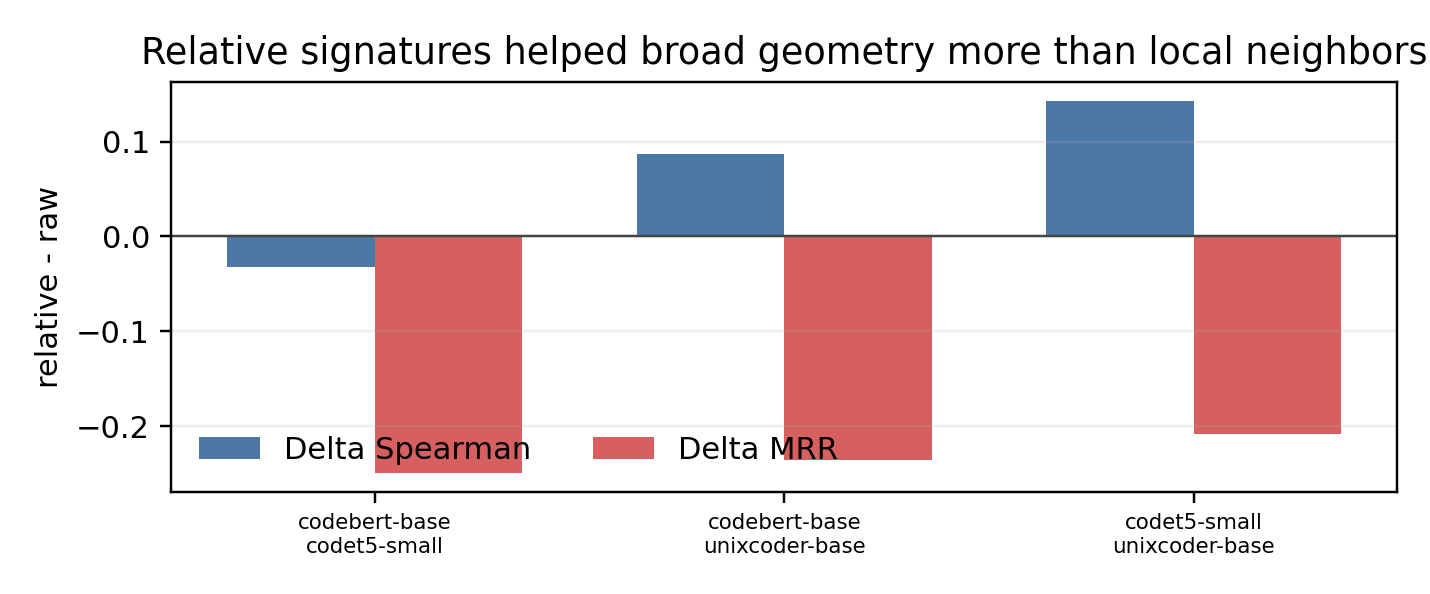
\includegraphics[width=0.78\linewidth]{figures/geometry_signal.png}
\caption{Relative signatures had some global-geometry signal, but local neighborhood preservation degraded. That was already a warning sign.}
\end{figure}

The takeaway was not ``this works.'' It was: there is structure in the relations, but not enough evidence that the raw relation space is a better search space.

\section*{Phase 2: Candidate Generation}

The next phase moved from direct replacement to candidate generation. Anchor ablations, learned-anchor variants, robustness checks, and LARP-style candidate recall all pointed the same way: the exact ordering was imperfect, but the candidate sets increasingly contained the correct neighbors.

This mattered. Search systems often do not need the first-stage retriever to be perfect. They need it to produce a small, high-recall pool for a more expensive reranker. In that role, relation signatures looked much less silly. Farthest anchors and row-zscored signatures were consistently better than naive random signatures. Learned anchor selection helped further. Multi-model tests reduced the chance that this was only a MiniLM accident.

The message became:

\begin{quote}
The retrieval ordering was imperfect, but the candidate sets increasingly contained the correct neighbors.
\end{quote}

Still, this was not the original claim. It was already a retreat.

\section*{Phase 3: Ridge Projection}

The main technical breakthrough was ridge-bilinear projection. Plain relation cosine assumed every anchor dimension should be compared with an identity metric. That was wrong. Some anchors were redundant. Some were noisy. Some only mattered through combinations.

Ridge projection treated relation signatures as coordinates, not as the final metric. Given relation signatures \(S\) and raw embeddings \(X\), it solved:
\[
W = (S^\top S + \lambda I)^{-1} S^\top X
\]
and searched projected relation vectors:
\[
z(x) = \mathrm{L2Norm}(s(x)W).
\]

This was the moment the project became genuinely interesting.

\begin{center}
\begin{tabular}{rcc}
\hline
Pool & Cosine & Ridge \\
\hline
10 & 0.6236 & 0.8314 \\
25 & 0.8176 & 0.9846 \\
50 & 0.9033 & 0.9975 \\
100 & 0.9534 & 0.9995 \\
250 & 0.9841 & 1.0000 \\
\hline
\end{tabular}
\end{center}

\begin{figure}[h]
\centering
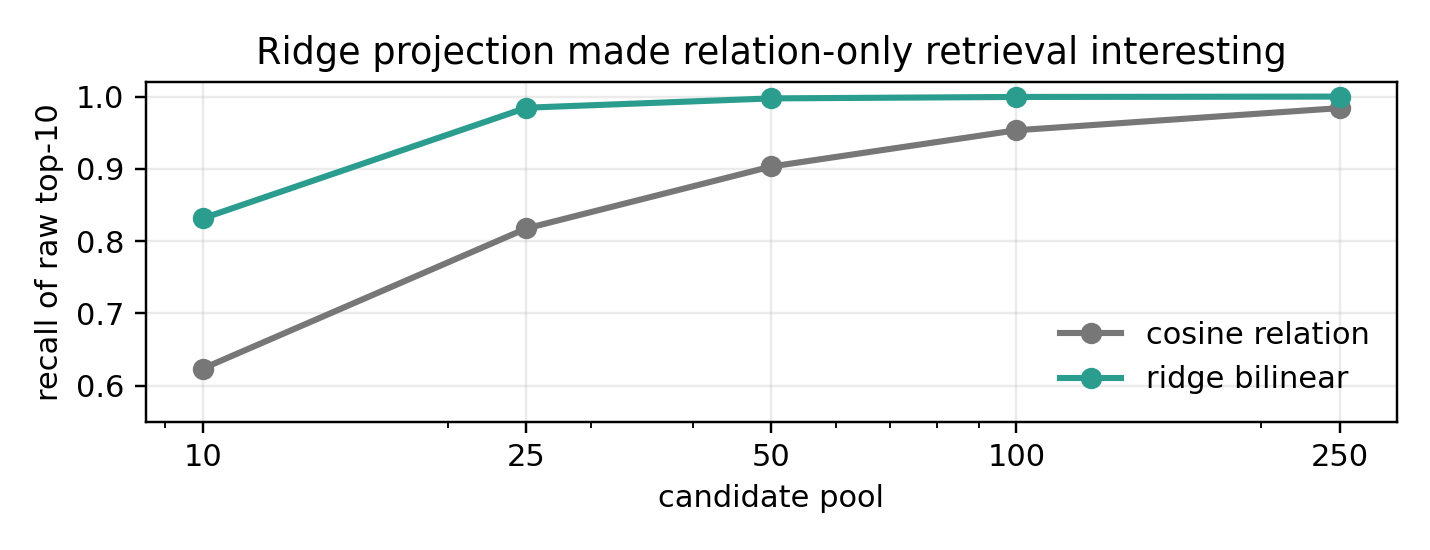
\includegraphics[width=0.78\linewidth]{figures/ridge_projection.png}
\caption{Ridge projection changed the relation space from a weak similarity heuristic into a strong candidate generator.}
\end{figure}

The important interpretation is not that ridge regression is novel. It is that the relation signature was not useless; it was a coordinate system that needed the right metric.

\section*{Phase 4: The Reality Check}

The direct-search comparison killed the strong version.

\begin{center}
\begin{tabular}{lcc}
\hline
System & 100k Recall@10 & 200k Recall@10 \\
\hline
raw\_hnsw & 0.9978 & 0.9924 \\
ridge\_relation\_hnsw & 0.9550 & 0.9584 \\
\hline
\end{tabular}
\end{center}

Raw HNSW won.

The relation index had similar vector memory, extra preprocessing, and lower direct top-k recall. It did not provide a compelling reason to replace raw search. The direct-replacement story died here.

\begin{figure}[h]
\centering
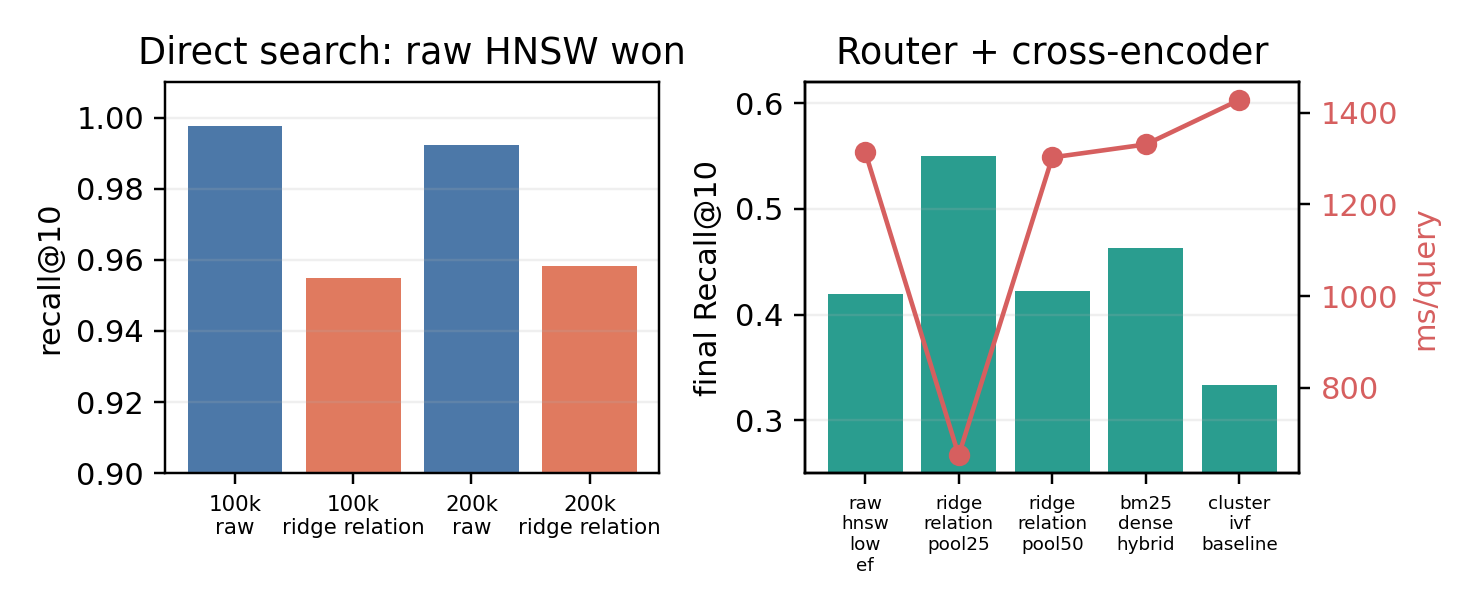
\includegraphics[width=0.92\linewidth]{figures/reality_router.png}
\caption{Left: raw HNSW won direct search. Right: relation routing survived only after the objective changed to routing plus reranking.}
\end{figure}

\section*{Phase 5: The Unexpected Result}

The final experiment changed the objective. Instead of asking whether relation signatures were a better nearest-neighbor index, it asked whether they were a better router before reranking.

Every system produced candidates. The same cross-encoder reranker then scored those candidates. The reranker was \texttt{cross-encoder/ms-marco-MiniLM-L-6-v2}, which is not code-specialized, so absolute quality should not be over-read. The comparison is still fair because every candidate source used the same reranker.

\begin{center}
\small
\begin{tabular}{lrrrrr}
\hline
System & Pool & Recall@10 & MRR@10 & NDCG@10 & Latency \\
\hline
raw\_hnsw\_low\_ef & 50 & 0.4200 & 0.8061 & 0.4800 & 1315 ms \\
ridge\_relation\_pool25 & 25 & 0.5500 & 0.8778 & 0.6008 & 652 ms \\
ridge\_relation\_pool50 & 50 & 0.4220 & 0.8048 & 0.4816 & 1303 ms \\
bm25\_dense\_hybrid & 50 & 0.4630 & 0.8262 & 0.5202 & 1331 ms \\
cluster\_ivf\_baseline & 50 & 0.3330 & 0.7505 & 0.3905 & 1428 ms \\
\hline
\end{tabular}
\end{center}

This is the first experiment where the relation layer won a benchmark that matters. It reranked half as many pairs as the 50-candidate systems, had lower latency, and produced better final Recall@10, MRR@10, and NDCG@10.

It won as infrastructure, not as retrieval.

\section*{What Actually Survived}

The defensible claims are limited:

\begin{itemize}
\item fixed-anchor signatures are stable under insertion,
\item candidate recall can become very high,
\item learned anchors help,
\item ridge projection matters,
\item relation signatures can act as semantic routing coordinates,
\item routing plus reranking is the strongest use case.
\end{itemize}

\section*{What Did Not Survive}

The dead ideas are equally clear:

\begin{itemize}
\item superior direct search backend,
\item raw-vector replacement,
\item universal cross-model preservation,
\item ``better HNSW.''
\end{itemize}

Those should not be revived without a new result that directly beats the relevant baseline.

\section*{Final Interpretation}

\begin{quote}
The project started as a search-index project and ended as a routing-layer project.
\end{quote}

The strongest version failed. The weaker version survived. The surviving version is probably the correct interpretation.

The relation representation did not replace raw embeddings. It did, however, become a useful way to route into a smaller reranking budget. That is less exciting than a new index, but it is more honest and maybe more product-relevant. A system that can route fewer candidates into an expensive reranker while preserving or improving final quality has a reason to exist.

\section*{Why I Stopped}

The central question was answered. Further tuning would mostly be optimization: better anchors, a code-specific reranker, FAISS instead of hnswlib, more datasets, different pool sizes. Those are valid engineering tasks, but they do not change the interpretation unless attached to a concrete product need.

There is enough evidence to stop treating this as a search-index replacement project. There is also enough evidence not to throw it away completely.

\begin{quote}
I am not continuing this unless there is a concrete routing/reranking use case.
\end{quote}

\end{document}
